\documentclass{article}
\usepackage{hyperref}
\usepackage{graphicx}
\begin{document}

\section{DECAM Information}
DECam has a three square degree field of view. 0.2637/0.2626 (arcsec/unbinned pixel). Large focal plane array with a close to circular array of 62 CCDs and a total of 520 million pixels. 
\newline 
CCD Array Characteristics:
\newline
Array Dimensions: 
    Axis 1: 2048 pixels
    Axis 2: 4096 pixels
\newline
Pixel Size: \SI{15}{\micro\metre}

\begin{figure}
    \centering
    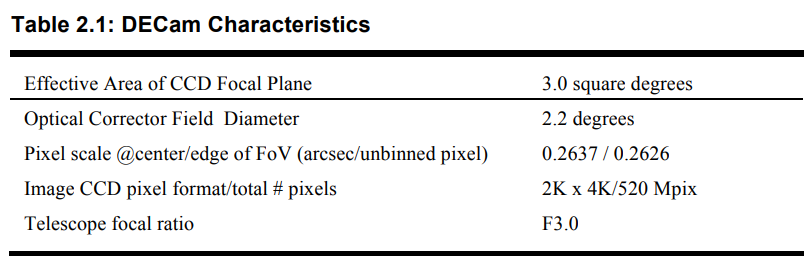
\includegraphics[width=0.5\linewidth]{Decam Characteristics.png}
    \caption{DECam Characteristics}
    \label{fig:enter-label}
\end{figure}

  \section{link dump}

  \href{https://github.com/cyb0rb/WiFeS_Catalog}{github repo}
  
  \href{https://sep.readthedocs.io/en/v1.1.x/tutorial.html}{source extractor tutorial}

\subsection{DECam}
  \href{https://astroarchive.noirlab.edu/api/docs/}{NOIRLab astro data archive}

  \href{https://github.com/NOAO/nat-nb/blob/master/sia.ipynb}{data archive query example notebook}

  \href{https://noirlab.edu/science/sites/default/files/media/archives/documents/scidoc0436.pdf}{DECam imager data handbook}
  
  \href{https://noirlab.edu/science/programs/ctio/instruments/Dark-Energy-Camera}{NOIRLab DECam information page} (has more links)
  
  \href{https://des.ncsa.illinois.edu/releases/other}{DES Data Management}
\end{document}